% \section{Introduction}
\begin{figure}
    \centering
    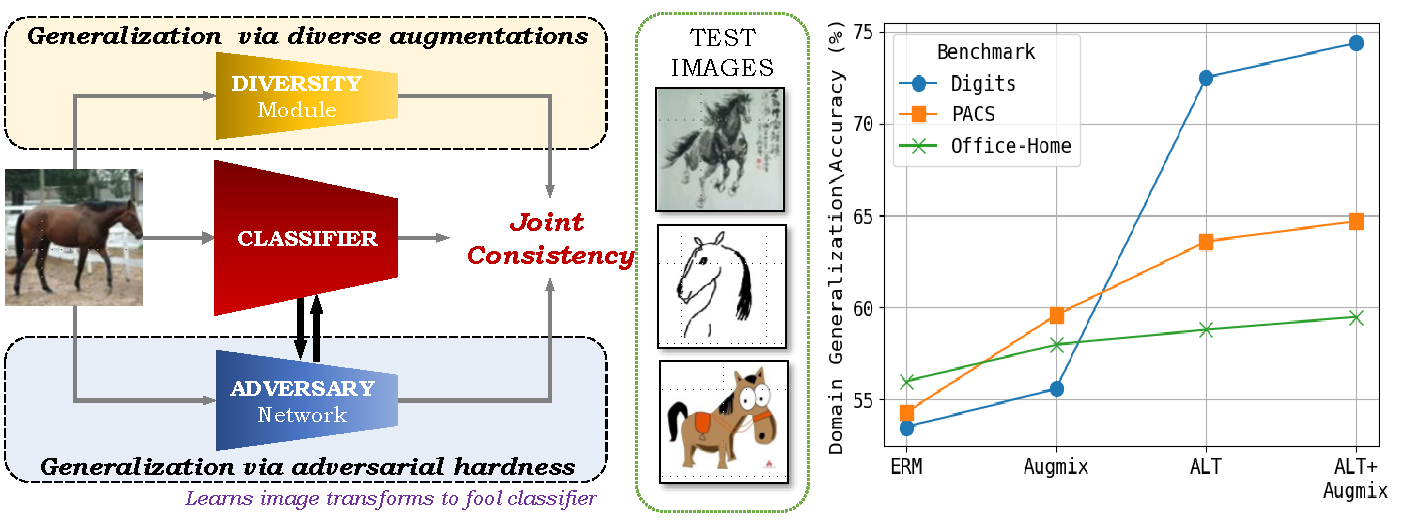
\includegraphics[width=\linewidth]{alt/figures/alt_teaser.pdf}
    \caption{
    This figure illustrates our approach which consists of a \textit{diversity} module (data augmentation functions such as Augmix~\citep{hendrycks2019augmix} or RandConv~\citep{xu2020robust}) and an \textit{adversary} network (ALT) (to learn image transformations that fool the classifier).
    We show an example from the PACS benchmark under the single-source domain generalization setting, with real photos (P) as the source domain and art paintings (A), cartoons (C), and sketches (S) as the target domains.
    The plot summarizes our results -- while diversity alone improves performance over the naive ERM baseline, adapting this diversity using adversarially learned transformations (ALT) provides a significant boost for domain generalization on multiple benchmarks.}
    \label{fig:alt_teaser}
\end{figure}


Domain generalization is the problem of making accurate predictions on previously unseen domains, especially when these domains are very different from the data distribution on which the model was trained. 
This is a challenging problem that has seen steady progress over the last few years \citep{carlucci2019domain,volpi2018generalizing,qiao2020learning,xu2020robust,nam2021reducing}. 
this chapter focuses on the special case -- single source domain generalization (SSDG) -- where the model has access only to a single training domain, and is expected to generalize to multiple different testing domains. 
This is especially hard because of the limited information available to train the model with just a single source. 

In the case where multiple training domains (i.e., multi-source DG) are available, recent analysis \citep{gulrajani2021in} shows that even simple methods like minimizing empirical risk jointly on all domains, performs better than most existing sophisticated formulations.
% on par with sophisticated formulations.
A corollary to this finding is that success in 
%SSDG
domain generalization is primarily dependent on \emph{diversity} -- i.e., exposing the model to as many potential training domains as possible.
As the SSDG problem allows access only to a single training domain, such an exposure must come in the form of diverse transformations of the source domain that can simulate the presence of multiple diverse domains ultimately leading to low generalization error. 
% which in this case must be in the form of diverse transformations of the source domain that can simulate the presence of multiple different domains ultimately leading to low generalization error. 

The idea of using diversity to train better models has been sufficiently explored -- many recent approaches have shown that a diverse set of augmentations during training improves a model's robustness under distribution shifts \citep{hendrycks2019augmix,yun2019cutmix,zhang2018mixup,cubuk2020randaugment}. 
However, the extent to which the model needs to be exposed to the diverse transformations is unclear, and over-exposure may hurt the model's generalization capabilities. 
Moreover, these methods define a strong prior in terms of the types of diversity that is desirable -- for e.g., in object recognition tasks, invariance to affine transformations, color jitter, blurs, or other kinds of pixel noise is desirable. 
Specific augmentations can be used if the type of diversity encountered at test time is known; for instance if it is known that the test set may contain random combinations of rotation, translation, and scaling, using augmentations that are correlated with this domain shift would lead good performance~\citep{gokhale2021attribute,benton2020learning,wong2020learning}.

Unfortunately, by design, these methods can only achieve invariance under small distribution shifts, like unknown corruptions, noise or imperceptible and perceptible adversarial attacks. 
These methods typically do not work effectively when the distribution shift is large and of a semantic nature, as in the case of domain generalization. 
On the other hand, some recent methods have directly used randomized convolutions to synthesize diverse image manipulations~\citep{xu2020robust}, motivated by the large space of potentially realizable functions induced by a convolutional layer, which cannot be easily emulated using simple analytical functions. 
 
In this chapter we hypothesize that, while diversity is critical in order to succeed in single domain generalization, diversity alone is insufficient. 
In other words, blindly exposing a model to a wide range of transformations cannot improve the generalization performance. Instead, we argue that other carefully designed forms of diversity are needed -- specifically those that can expose the model to unique, and task-dependent transformations with large semantic changes that are otherwise unrealizable with plug-and-play augmentations as before.  To this end, we introduce an adversary network whose objective is to find plausible image transformations that maximize classification error. We enforce a consistency between a \textbf{diversity module} and the \textbf{adversary network} during training along with the classifier's predictions. 

Our method, dubbed ALT (adversarially learned transformations), offers an interplay between diversity and adversity. Over time, a synergistic partnership between the diversity and adversary networks emerges, exposing the model to increasingly unique, challenging and semantically diverse examples that are ideally suited for single source domain generalization.  The adversary network benefits from the classifier being exposed to the diversity module, and as such avoid trivial adversarial samples with appropriate checks. This allows the adversarial maximization to explore a wider space of adversarial transformations that cannot be covered by prior work on pixel-level additive perturbations.
  
We demonstrate this advantage of our method empirically on multiple benchmarks -- PACS \citep{li2017deeper}, Office-Home \citep{venkateswara2017deep}, and Digits \citep{volpi2018generalizing}. On each benchmark, we outperform the state-of-the-art single source domain generalization methods by a significant margin.  Moreover, since our framework disentangles diversity and adversarial modules, we can combine it with various diversity enforcing techniques -- we identify two such state-of-the-art methods with AugMix \citep{hendrycks2019augmix}, and RandConv \citep{xu2020robust}, and show that placing them inside our framework leads to significantly improved generalization performance over their vanilla counterparts. 
We illustrate this idea in figure \ref{fig:alt_teaser} where we show an image of a horse from the 'photo' training distribution in PACS and the different styles of cartoon/sketch/art painting horses that may be encountered at test time. 

\paragraph{Contributions:}
We summarize our contributions below:
\begin{itemize}[nosep,noitemsep,leftmargin=*]
    \item We introduce a method, dubbed ALT, which produces adversarially learned image transformations that expose a classifier to a large space of image transformations for superior domain generalization performance. ALT performs adversarial training in the parameter space of an adversary network as opposed to pixel-level adversarial training.
    \item We show how ALT integrates diversity-inducing data augmentation and hardness-inducing adversarial training in a synergistic pipeline, leading to diverse transformations that cannot be realized by blind augmentation strategies or adversarial training methods on their own.
    \item We validate our methods empirically on three benchmarks demonstrating state-of-the-art performance, and provide insights into and analysis of approach.
\end{itemize}

% Instead, the model must be able to trade-off diversity and classifier performance as needed such that it achieves 'optimal' exposure in a given task, and no more --  which is challenging to define \emph{a priori}. Instead, we are able to achieve this trade-off using a consistency using an additional network that acts an adversary to the classifier by learning adversarial transformations of the input image for every single batch during training. By randomly initializing this network in each iteration, we ensure the adversarial transformations are unique, and diverse themselves. We then place a consistency objective between the diverse and adversarial transformations so together they expose the model to learn from both diverse and challenging domains